\section*{Transformers}

- A transformer is a neural network that iteratively transforms a sequence to another sequence and mixes the information between the sequence elements via self-attention.

\subsection*{Architecture}


\begin{wrapfigure}{r}{0.4\columnwidth} 
    \centering
    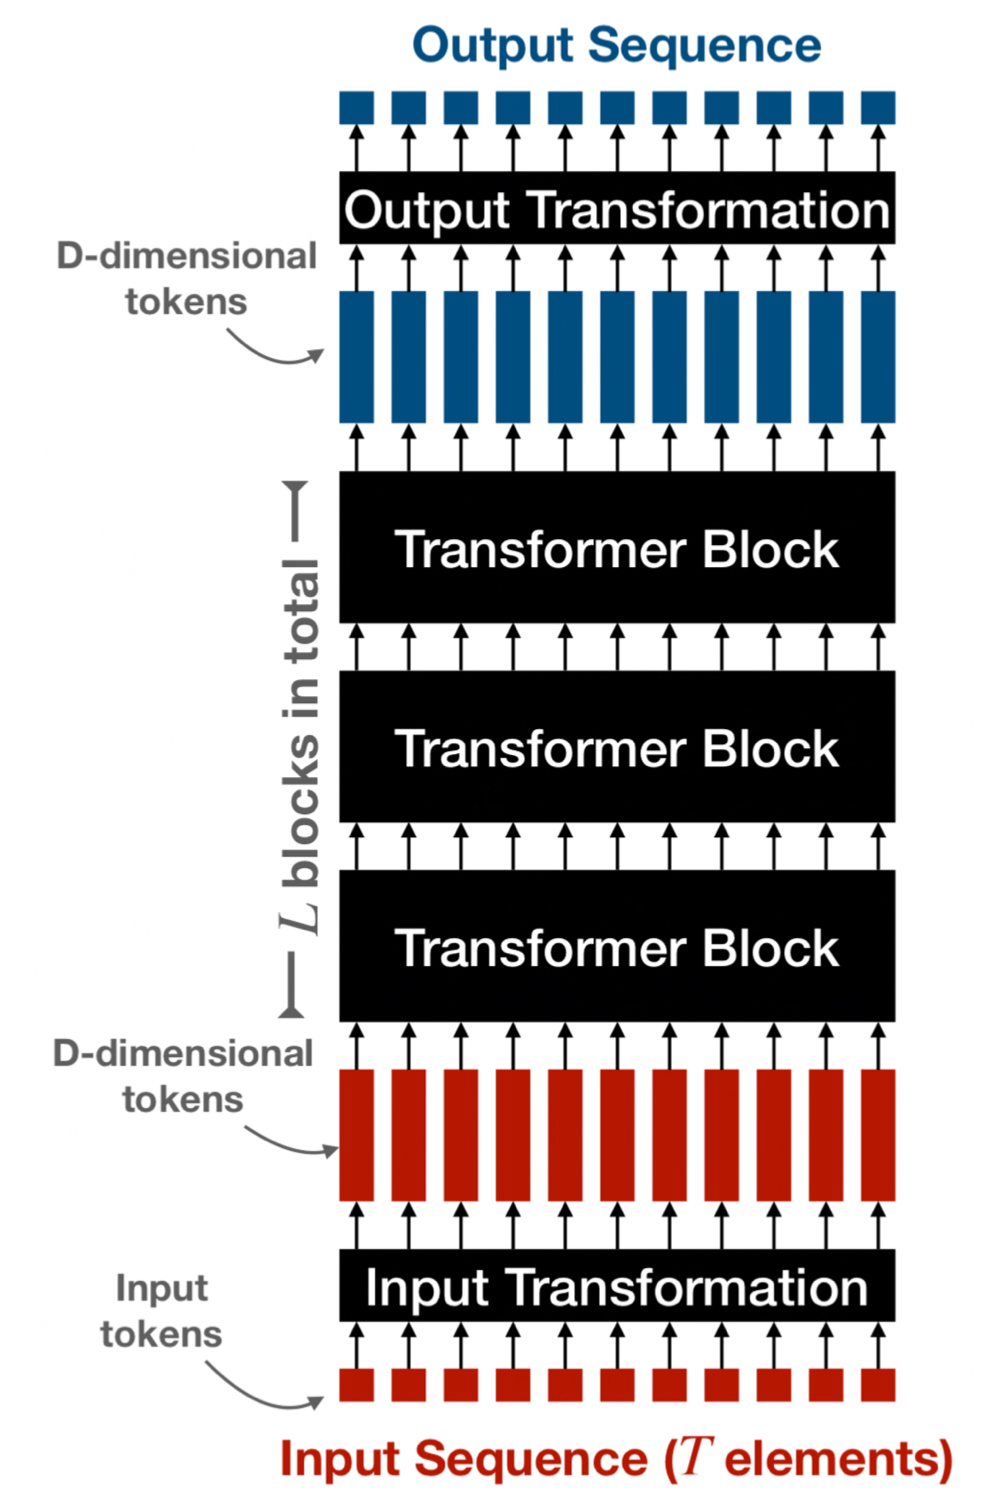
\includegraphics[width=0.4\columnwidth]{figures/transformer_architecture.jpeg}
    \vspace{-10pt}
\end{wrapfigure}

- Self-Attention (SA): mixes information between tokens

- Multi-Layer Perceptron (MLP): mixes information within each token

- Skip connections are widely used

- Layer normalization (LN) is usually placed at the start of a residual branch

\begin{wrapfigure}{l}{0.2\columnwidth}
  % \centering
  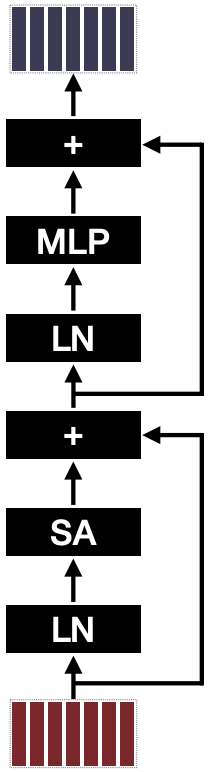
\includegraphics[width=0.2\columnwidth]{figures/transformer_block.png}
%   \caption{}
%   \label{fig:cfm_pca2D_wrapped}
\end{wrapfigure}

\subsection*{Text Token Embeddings}

- Tokenization: split the input text into a sequence of input tokens (typically word fragments + some special symbols) according to some predefined tokenizer procedure: 

- Convert each token ID $i\in\{1,...,N_{vocab}\}$ into a real-valued vector $\mathbf{w}_{i}\in\mathbb{R}^{D}$

- This can be seen as a matrix multiplication $\mathbf{W}\cdot\mathbf{e}_{i}=\mathbf{W}_{:,i}=\mathbf{w}_{i}{\mathrm{~(with~\mathbf{W}\in\mathbb{R}^{D \times N_{vocab}}}})$


- $\mathbf{W}$ is learned via backpropagation, along with all other transformer parameters (however, the tokenizer procedure is typically fixed in advance and not learned)

- The whole input sequence of $T$ tokens leads to an input matrix $X\in\mathbb{R}^{T\times D}$

\subsection*{Attention}

- Attention is a function that transforms a sequence of tokens to a new sequence of tokens using a learned input-dependent weighted average

- Input tokens : $V\in\mathbb{R}^{T_{i n}\times D}$

- Output tokens : $Z\in\mathbb{R}^{T_{out}\times D}$

- Output tokens are simply a weighted average of
the input tokens:
$z_{i}=\sum_{j=1}^{T_{i}}p_{i j}v_{j}$ i.e. $Z=P V$

- Weighting coefficients ${\cal P}\in[0,1]^{T_{out}\times T_{i n}}$ form valid probability distributions over the input tokens $\textstyle\sum_{j=1}^{T_{i n}}p_{i j}=1$

- Query tokens : $Q\in\mathbb{R}^{T_{out}\times D_{K}}$

- Key tokens : $K\in\mathbb{R}^{T_{in}\times D_{K}}$

- Determine weight $p_{i,j}$ based on how simmilar $q_i$ and $k_j$ are.

- Use inner product to obtain raw similarity scores.

- Normalize with softmax (scaled the temperature by $\sqrt{D_{K}}$) to obtain a probability distribution.

- $P=\mathrm{softmax}\left({\frac{Q K^{\mathsf{T}}}{\sqrt{D_{K}}}}\right)$ The softmax is applied on each row independently. Scaling ensures uniformity
at initialization and faster convergence

\subsection*{Self-Attention}

\begin{wrapfigure}{r}{0.4\columnwidth}
  % \centering
  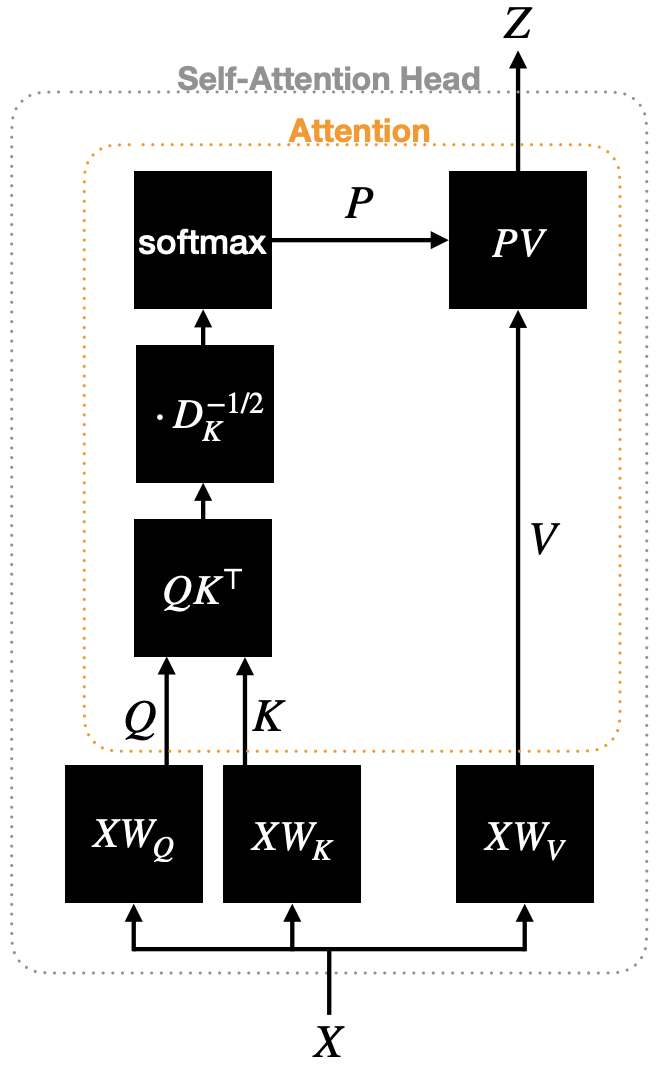
\includegraphics[width=0.4\columnwidth]{figures/self_attention.png}
%   \caption{}
%   \label{fig:cfm_pca2D_wrapped}
\end{wrapfigure}

- $V,K,Q$ are all derived from the same input token
sequence $X\in\mathbb{R}^{T\times D}$

- Values : $V=X W_{V}\in\mathbb{R}^{T\times D},\,W_{V}\in\mathbb{R}^{D\times D}$

- Keys : $K=X W_{K}\in\mathbb{R}^{T\times D_{K}},\,W_{K}\in\mathbb{R}^{D\times D_{K}}$

- Queries : $Q=X W_{Q}\in\mathbb{R}^{T\times D_{K}},W_{Q}\in\mathbb{R}^{D\times D_{K}}$

- $W_{Q},\,W_{V},\,W_{K}$ are learned parameters.

- $Z=\mathrm{softmax}\left(\frac{X W_{Q}W_{K}^{T}X^{T}}{\sqrt{D_{K}}}\right)X W_{V}$

\subsubsection*{Multi-Head Self-Attention}

\begin{wrapfigure}{r}{0.3\columnwidth} 
  \centering
  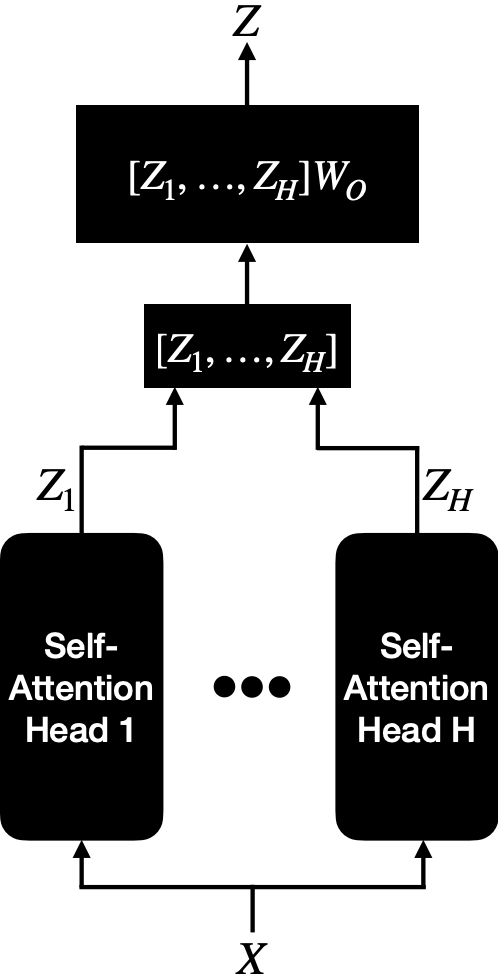
\includegraphics[width=0.3\columnwidth]{figures/multi_head.png}
\end{wrapfigure}

- Run $H$ Self-Attention “heads” in parallel

- $Z_{h}={\mathrm{softmax}}\left({\frac{X W_{Q,h}W_{K,h}^{\mathsf{T}}X^{\mathsf{T}}}{\sqrt{D_{K}}}}\right)X W_{V,h}\in\mathbb{R}^{T\times D_{V}}$ 


- $W_{V,h}\in\mathbb{R}^{D\times D_{V}},\,W_{K,h}\in\mathbb{R}^{D\times D_{K}},\,W_{Q,h}\in\mathbb{R}^{D\times D_{K}}$

- The final output is obtained by concatenating head-outputs and applying a linear transformation $Z=[Z_{1},\dots,Z_{H}]W_{o}$ where $W_{O}\in\mathbb{R}^{H D_{V}\times D}$ is learned via backpropagation
% \lipsum[1]

\subsection*{Positional Information}

- Attention by itself does not account for the order of input

- incorporate a positional encoding in the network which is a function from the position to a feature vector $p o s:\left\{1,...,T\right\}\rightarrow\mathbb{R}^{D}$

- The most basic choice is to add a positional embedding $W_{p o s}$ corresponding to each token's position $t$ to the input embedding. $W_{p o s}\in\mathbb{R}^{D\times T}$ is learned via backpropagation along with the other parameters

\subsection*{MLP}

- Mixing Information within Tokens

- Apply the same transformation to each token
independently: $M L P(X)=\varphi(X W_{1})W_{2}$

- $W_{1},W_{2}\in\mathbb{R}^{D\times D}$ learned via backprop

\subsection*{Output Transformations}

- typically simple: linear
transformation or a small MLP

- dependent on the task: Single output (e.g.,sequence-level classification): apply an output transformation to a special taskspecific input token or to the average of all tokens. Multiple outputs (e.g., per-token classification): apply an output transformation to each token independently

\subsection*{Vision Transformer Architecture}

- Self-attention is more general than convolution and can potentially express it

- The receptive field is the whole image after just one self-attention layer

- ViTs require more data than CNNs due to their reduced inductive bias in extracting local features

- In many cases, the model attends to image regions that are semantically relevant for classification

\subsection*{Encoders \& Decoders}

\begin{wrapfigure}{r}{0.3\columnwidth} 
  \centering
  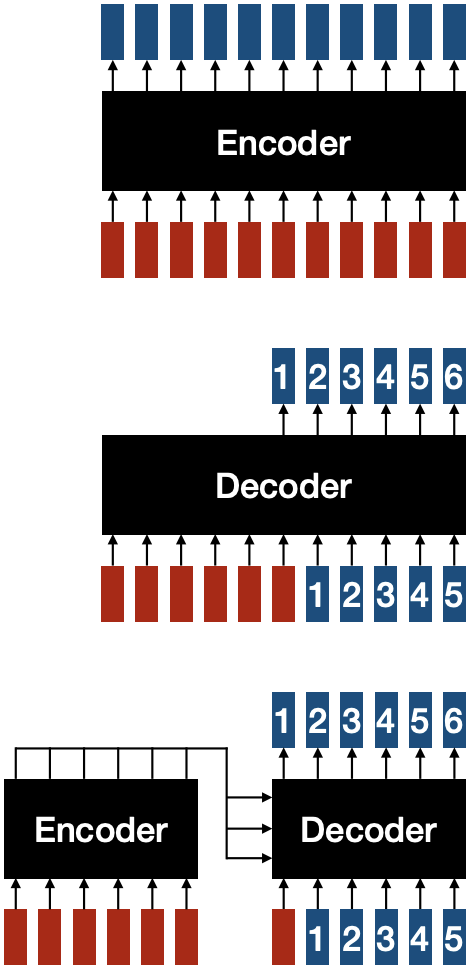
\includegraphics[width=0.3\columnwidth]{figures/encoders_decoders.png}
\end{wrapfigure}

- Encoders (e.g., classification): They produce a fixed output size and process all inputs simultaneously

- Decoders (e.g., ChatGPT): Auto-regressively sample the next token as $x_{t+1}\sim s o f i m a x(f(x_{1},....,x_{t}))$ and use it as new input token. Capable of generating responses of arbitrary length.

- Encoder-decoder (e.g., translation): First encode the whole input (e.g., in one language) and then decode to token by token (e.g., in a different language)
